\documentclass{article}

\usepackage{pdfsync}
\usepackage{natbib}
\usepackage{hyperref}
\usepackage{graphicx}
\usepackage{caption}
\usepackage{subcaption}

% dot graphs
\usepackage{dot2texi}
\usepackage{tikz}
\usetikzlibrary{shapes,arrows}

\begin{document}
	\author{Robin Deits\\ rdeits@csail.mit.edu}
	\title{6.375 Report: Adaptive PIV: Synthesis}
	\date{\today}
	\maketitle

	\tableofcontents

	\section{Overview}
	This project is designed to implement Particle Image Velocimetry (PIV) on hardware, using an FPGA. The purpose is to allow for real-time analysis of fluid flows using optical tracking of thousands of particles. Specifically, this project introduces a framework for PIV on hardware which allows for adaptive selection of interrogation windows, which can improve the flow resolution in the busiest parts of the fluid. 

	\section{Background: PIV} % (fold)
	\label{sec:background}
	Particle Image Velocimetry (PIV) is an optical approach to measuring the flow field of a fluid, and has been used in the study of combustion, water flow, robotics, and many other fields. It involves seeding a fluid with tracking particles and using a laser or other planar lighting system to capture sequential images of the particle positions in a single thin 2D slice of the fluid. By comparing the change in position of groups of particles between the subsequent frames, a measurement of the local flow vector can be computed for each region of the fluid. This process of determining the movement of each section of the image is extremely time-consuming in a sequential programming system, but can be readily parallelized to significantly improve performance \citep{Yu:2006tb}

	Each PIV computation is performed on a pair of sequential images. Computation of the fluid flow begins by dividing the image up into small windows of, for example, 64px on a side. A small window size helps ensure that all of the particles within the window move with the same velocity between the two frames. For each window, we extract the subimage corresponding to that window from the first image in the pair. We will call this subimage $A$. We then extract a set of subimages $B_{\Delta x,  \Delta y}$ by shifting the original window in two dimensions and extracting the corresponding subimages from the second image in the pair. We can then perform a cross-correlation between $A$ and each $B_{i, j}$ and determine the shift in $x$ and $y$ which maximizes the correlation. This gives the most likely location of the particles from window $A$ in the second frame, and thus indicates the movement of that section of the fluid between the frames.
	% section background (end)

	\section{Adaptive PIV} % (fold)
	\label{sec:adaptive_piv}
	Standard PIV algorithms involve an even spatial distribution of interrogation windows $A$ with a fixed window size and some fixed overlap, such as 64\,px windows beginning every 16\,px. However, in order to achieve sufficient accuracy in busy fluid flows, it can be necessary to choose very small windows or very high degrees of overlap, which increases the computational demands by requiring far more cross-correlation computations. 	Theunissen et al. proposed a method for improving the performance of PIV in sub-optimial conditions, called Adaptive PIV \citep{Theunissen:2009cr}. Their method uses information about the current density of seeding particles and the prior estimate of the velocity field to update the size and spatial frequency of the interrogation windows $A$. This has the effect of increasing the number of data points in the busiest (highest particle density and highest velocity) parts of the fluid and reducing the number of samples in the most stable areas of the fluid, which can improve the amount of relevant data collected per computational unit. 

	In this project, I will focus on implementing Adaptive PIV on an FPGA to improve computational performance, with the ultimate goal of allowing accurate real-time fluid tracking. I will be expanding on prior work implementing a standard PIV algorithm on an FPGA \citep{Yu:2006tb}. I will also be using a recent \textsc{Matlab} implementation of the Adaptive PIV algorithm by Samvaran Sharma of the Robot Locomotion Group at MIT CSAIL as the reference code for my implementation. 

	The primary benefit of this project should be the parallelization and speedup of the Adaptive PIV algorithm. In order to achieve the desired image size and accuracy, Sharma's current software requires approximately 2.5 seconds per pair of frames, which makes real-time analysis of the fluid flow impossible. In contrast, Yu et al. were able to compute 15 image pairs per second using their FPGA implementation. My goal will be to achieve this result with the added benefits of the adaptive algorithm's focus on the most important areas of the fluid flow.
	% section adaptive_piv (end)

	\section{Target Application}
	\label{sec:target_app}
	The target application of this system is to perform PIV tracking on camera data in real time. This means processing 15 pairs of images per second (for a 30\,Hz overall framerate). I address the feasibility of this throughput in Section \ref{sec:computation}. 

	The ability to perform real-time PIV using a customized hardware system would be of great value to a project such as the MIT RoboClam, with which I have spent several years working. This project seeks to understand and replicate the efficient burrowing mechanism of the Atlantic razor clam, \emph{Ensis directus}, in order to create self-digging anchors for energy-constrained underwater vehicles. The razor clam uses the contraction of its shell to unpack the substrate around it, making digging much easier \citep{Winter:2012hj}. We use PIV to analyze the motion of both the real animal and its robotic counterpart and the effects that their motions have on the surrounding substrate. Adding real-time PIV would enable rapid feedback about the effects the robot is having on the substrate as we design and improve its motion patterns. 

	\section{Implementation}
	I have divided the implementation of the PIV system up into the high-level logic, which is performed in Python, and the computationally intensive and parallelizable cross-correlation which is performed on the FPGA. This division is shown in Figure~\ref{fig:system}. The host machine reads image pairs from disk (simulating live capture from a camera system), then converts them to 4-bit grayscale. These image pairs are transmitted over SCEMI to the FPGA, which stores both images in Block RAM. The host machine then selects a series of interrogation windows. The exact method of selection will depend on whether we are performing normal or adaptive PIV. The host transmits the coordinates of the interrogation windows to the DUT. The FPGA then extracts the actual image data for each window, performs the cross-correlation, and locates the peak in the cross-correlation value signifying the displacement of the particles in the window. The FPGA then sends the displacement back to the host. 

	\subsection{Module: PIV}
	The PIV master module handles all input and output operations to the SceMi layer and manages access to the primary Block RAM. Image data is passed into the PIV in packets of 8 pixels, in order to improve transmission performance across SceMi. The PIV master breaks up the packets into individual pixels and stores them in RAM. When the host sends a request for a particular interrogation window, the PIV master chooses the next available Window Tracker and downloads the sub-frames corresponding to the desired pixel coordinates of the window to the Window Tracker's own Block RAM. Once that tracker has finished computing the displacement of its window, the PIV master returns the displacement data to the host.

	\subsection{Module: Window Tracker}
	The FPGA program contains many instances of the Window Tracker module, each of which performs the cross-correlation and displacement extraction for a single interrogation window. The Window Tracker has a number of submodules, described below:

	\subsubsection{Module: Window Manager}
	The Window Manager is responsible for storing the entire sub-frame from each of the source images for a particular interrogation window. Data is fed into the Window Manager from the PIV master when a particular window is requested. Once that download is complete the Window Manager begins to output each pair of pixels which must be multiplied as part of the cross-correlation computation. 

	\subsubsection{Module: Accumulator}
	The Accumulator takes pixel values from the Window Manager and computes a running sum of the product of its pairs of inputs. It automatically resets its internal total to zero for each element in the cross-correlation matrix output. Since its operation is fully pipelined, it needs only a FIFO of pixel pairs from the Window Manager and a FIFO of cross-correlation matrix elements to send to the Displacement Tracker. 

	\subsubsection{Module: Displacement Tracker}
	The Displacement Tracker determines from the output of the Accumulator the current displacement values with the highest cross-correlation between the windows. It reads cross-correlation elements from the output FIFO of the Accumulator and maintains internal variables for the highest result seen so far and the x and y displacements corresponding to it. Once all cross-correlation computations are finished, it makes its result available. 


\begin{figure}[htbp]
\makebox[\textwidth][c]{
	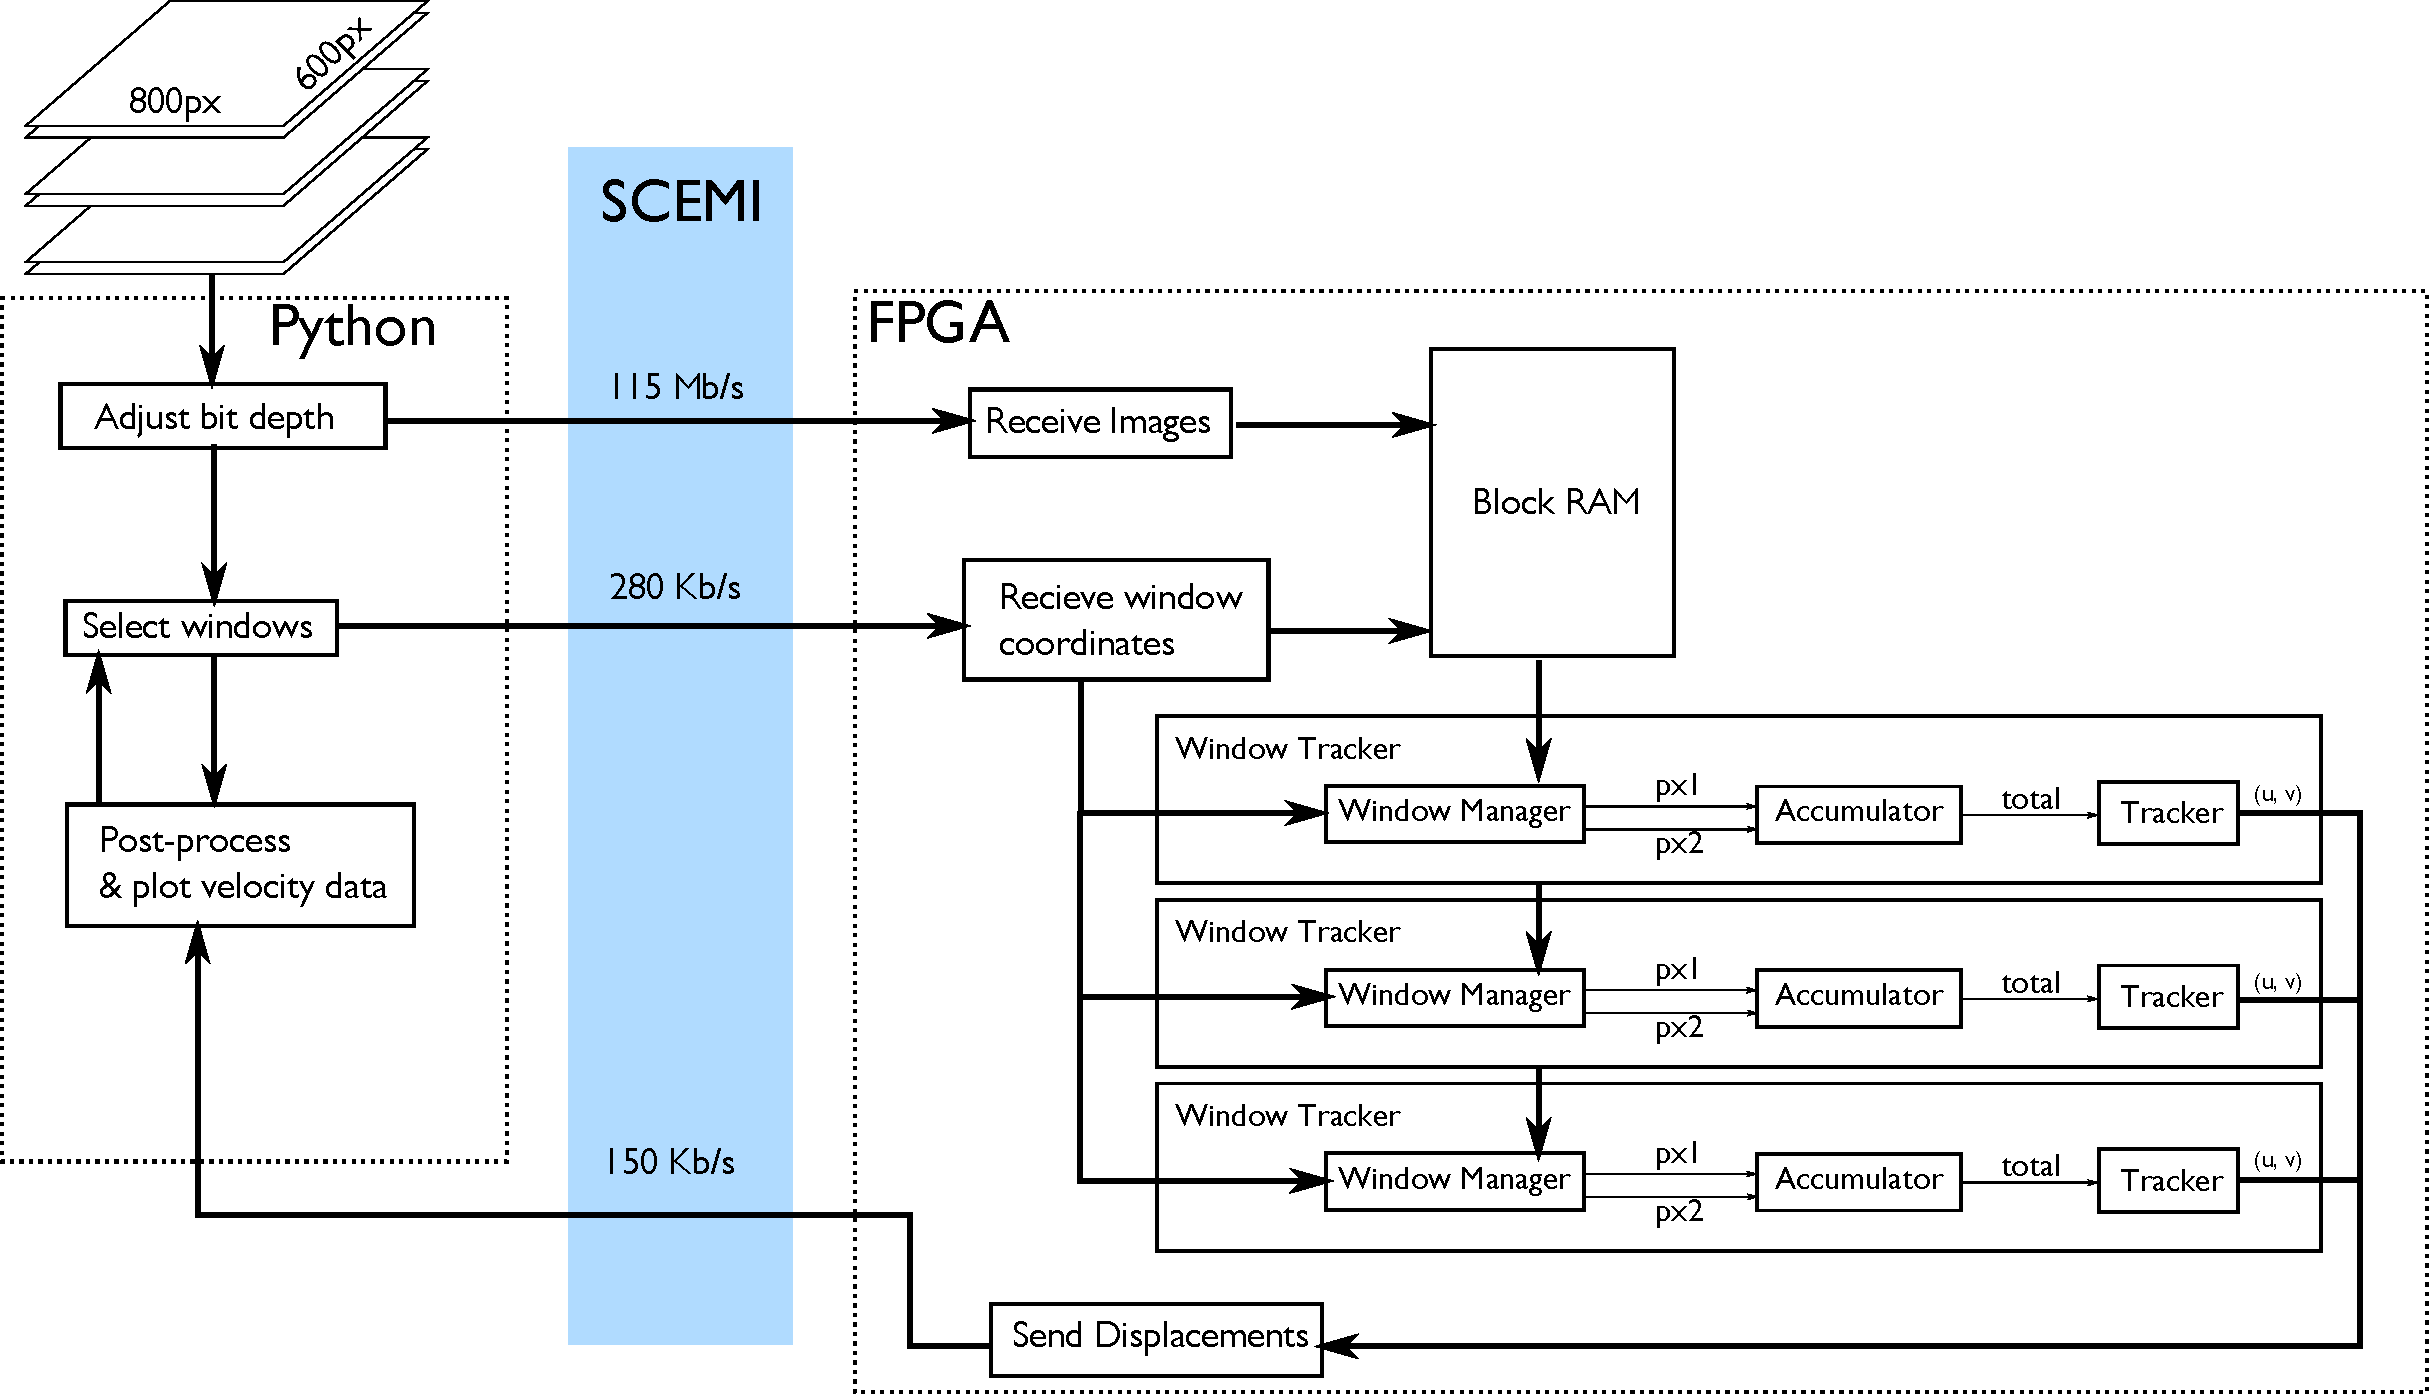
\includegraphics[width=1.4\textwidth]{fig/system_diagram.pdf}}
	\caption{The system diagram for the Adaptive PIV implementation on the FPGA. High-level logic relating to the particular PIV implementation is performed in Python, and the cross-correlation is performed on the FPGA. Only 3 Window Tracker modules are shown, but the full implementation should have up to 40 or more.}
	\label{fig:system}
\end{figure}

\section{Computational Requirements}
\label{sec:computation}
This section describes the computational goals of the PIV implementation. I will discuss the actual performance of the system and how it relates to these goals in Section \ref{sec:performance}. In order to assess the computational requirements of this design, I chose to use the interrogation window parameters presented by Yu et al. \citep{Yu:2006tb}. This choice means an interrogation window of 40x40px for the first image in each pair and 32x32px for the second image in each pair. For clarity, we will refer to the images as Image A and Image B and the frames as Frame A (40x40) and Frame B (32x32). Cross-correlation will be performed for each fully overlapping position of Frame B within Frame A. This means that the cross-correlation matrix will have $(40 - 32 + 1) ^2 = 81$ elements. 

Each element in the cross-correlation matrix will require $32 * 32$ multiplications and additions, so the entire cross-correlation matrix will require $32 * 32 * 81 = 82944$ multiplications. To compute the full velocity vector field for normal PIV, using an 8 pixel shift between interrogation windows, we must compute 1680 cross-correlation matrices per image pair. This means that, for a throughput of 15 image pairs per second, we need to perform $2,090,188,800$ multiplications per second. At a clock speed of 50\,MHz, that comes down to approximately 40 multiplications per clock cycle, meaning that the final design will need 40 Window Tracker modules each performing a single multiplication per cycle. 

\section{Demonstration}
To test the PIV system, I generated several small image pairs with known displacements. By applying an 80x60\,px window to a source image, and then shifting that window by a few pixels in a given direction, I created pairs of images with perfectly uniform, controlled displacements, which the PIV system was able to accurately track. One such pair is shown in Figure \ref{fig:diag_test}. 

In addition, I have run the PIV system in simulation on an entire 800x600\,px image pair, using the test set from Sharma's adaptive PIV system. The results are shown  in Figure \ref{fig:full_test}. 

\begin{figure}
	\centering
	\begin{subfigure}[htb]{0.45\textwidth}
		\centering
		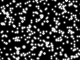
\includegraphics[width=\textwidth]{../../data/test/x+2_y+2/A.png}
	\end{subfigure}
	\begin{subfigure}[htb]{0.45\textwidth}
		\centering
		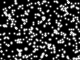
\includegraphics[width=\textwidth]{../../data/test/x+2_y+2/B.png}
	\end{subfigure}

	\begin{subfigure}[htb]{.7\textwidth}
		\centering
		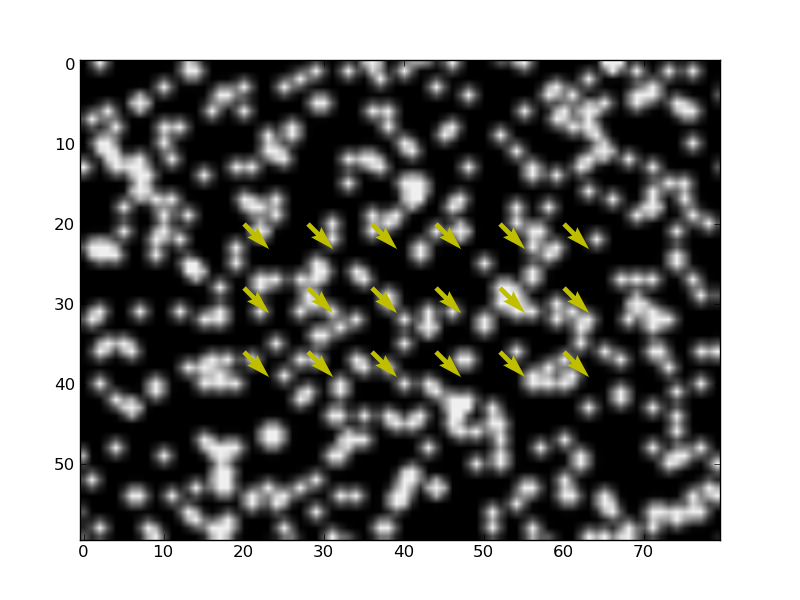
\includegraphics[width=\textwidth]{fig/x+2_y+2_PIV.png}
	\end{subfigure}
	\caption{A pair of sample images created to test the PIV system. The image on the upper left has been shifted down and to the right by two pixels to create the image on the upper right. The lower image shows the calculated flow field from the PIV program, which matches this displacement.}
	\label{fig:diag_test}
\end{figure}

\begin{figure}
	\centering
	\begin{subfigure}[htb]{0.45\textwidth}
		\centering
		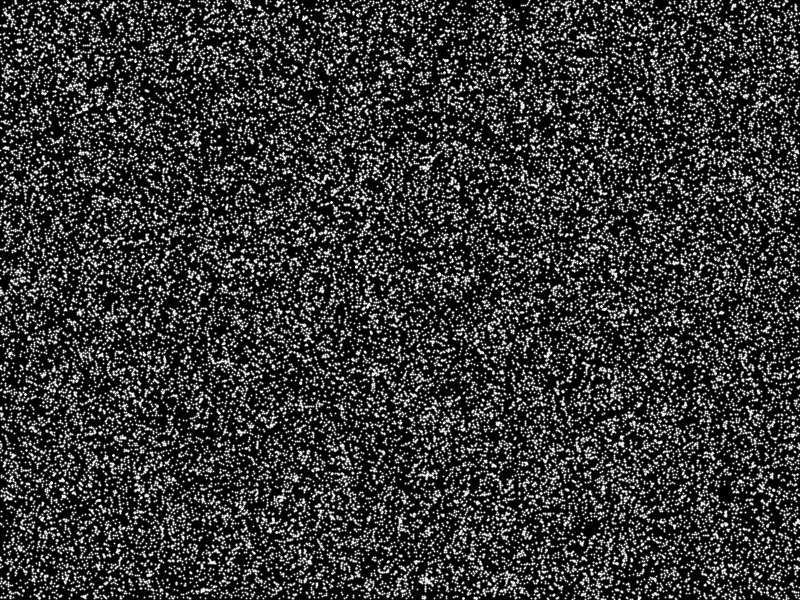
\includegraphics[width=\textwidth]{../../data/vort_sim/A.png}
	\end{subfigure}
	\begin{subfigure}[htb]{0.45\textwidth}
		\centering
		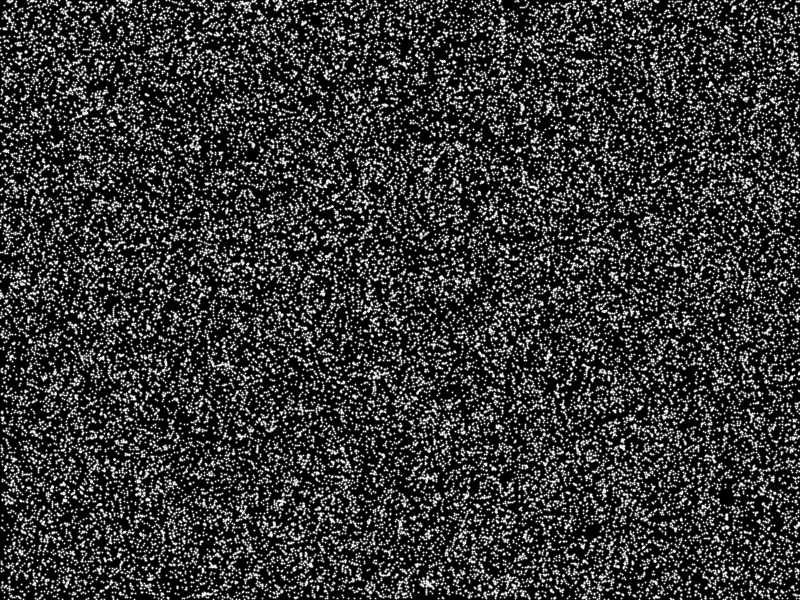
\includegraphics[width=\textwidth]{../../data/vort_sim/B.png}
	\end{subfigure}

	\begin{subfigure}[htb]{\textwidth}
		\centerline{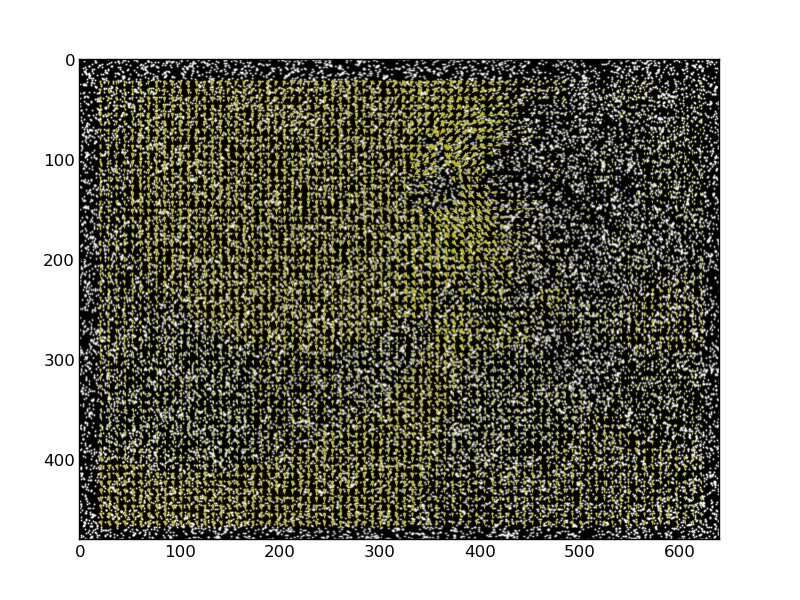
\includegraphics[trim = .4in .4in .4in .4in, clip, width=1.5\textwidth]{fig/vort_sim_non_adapt.png}}
	\end{subfigure}
	\caption{A pair of full-size synthetic images taken from Sharma's adaptive PIV system, along with the measured flow field from the simulated FPGA implementation.}
	\label{fig:full_test}
\end{figure}

\subsection{Demonstrating Adaptive PIV}
To demonstrate that this system is flexible enough to handle an adaptive PIV wrapper, with no changes to the FPGA program, I created a simple Python application to request windows with variable spatial frequency. Using velocity data compiled from a previous run, I generated a probability density map based on total velocity at each point in the image, then sampled 1000 window locations from this distribution. The density and the resulting sampled points can be seen in Figure \ref{fig:distribution}. 

\begin{figure}
	\centering
	\begin{subfigure}[htb]{0.45\textwidth}
		\centering
		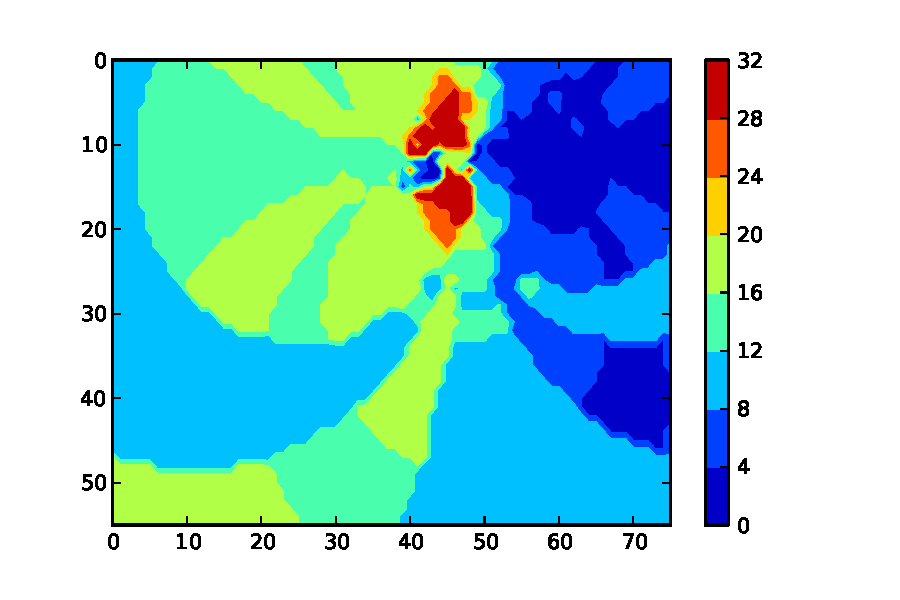
\includegraphics[width=\textwidth]{fig/sample_density.pdf}
	\end{subfigure}
	\begin{subfigure}[htb]{0.45\textwidth}
		\centering
		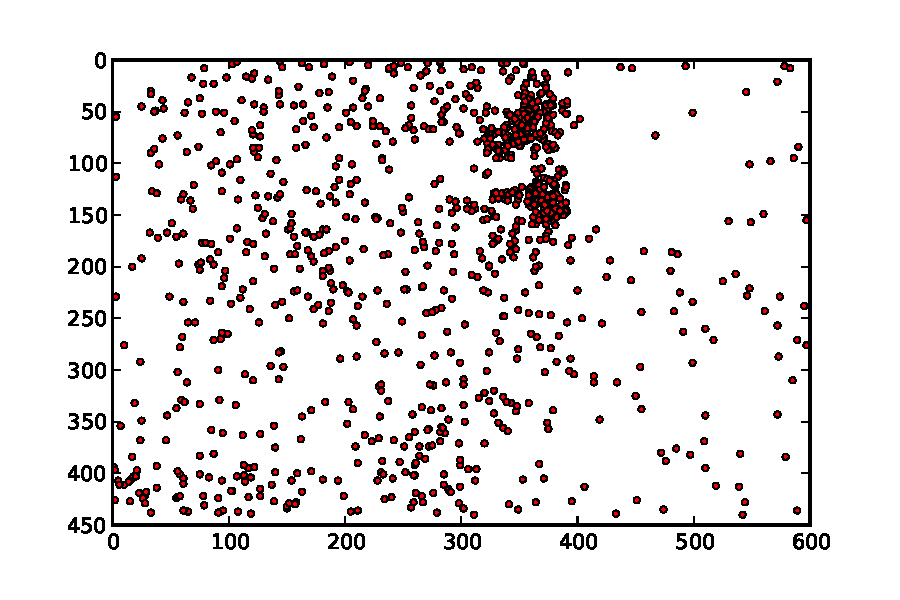
\includegraphics[width=\textwidth]{fig/sample_points.pdf}
	\end{subfigure}
	\caption{Sampling distribution created from prior fluid flow estimate (a) and interrogation window locations drawn from that distribution (b). Note the high probability density in the top-center of the image, where the vortex shown in Figure \ref{fig:full_test} is located.}
	\label{fig:distribution}
\end{figure}

\begin{figure}
	\centering
	\begin{subfigure}[htb]{0.8\textwidth}
		\centering
		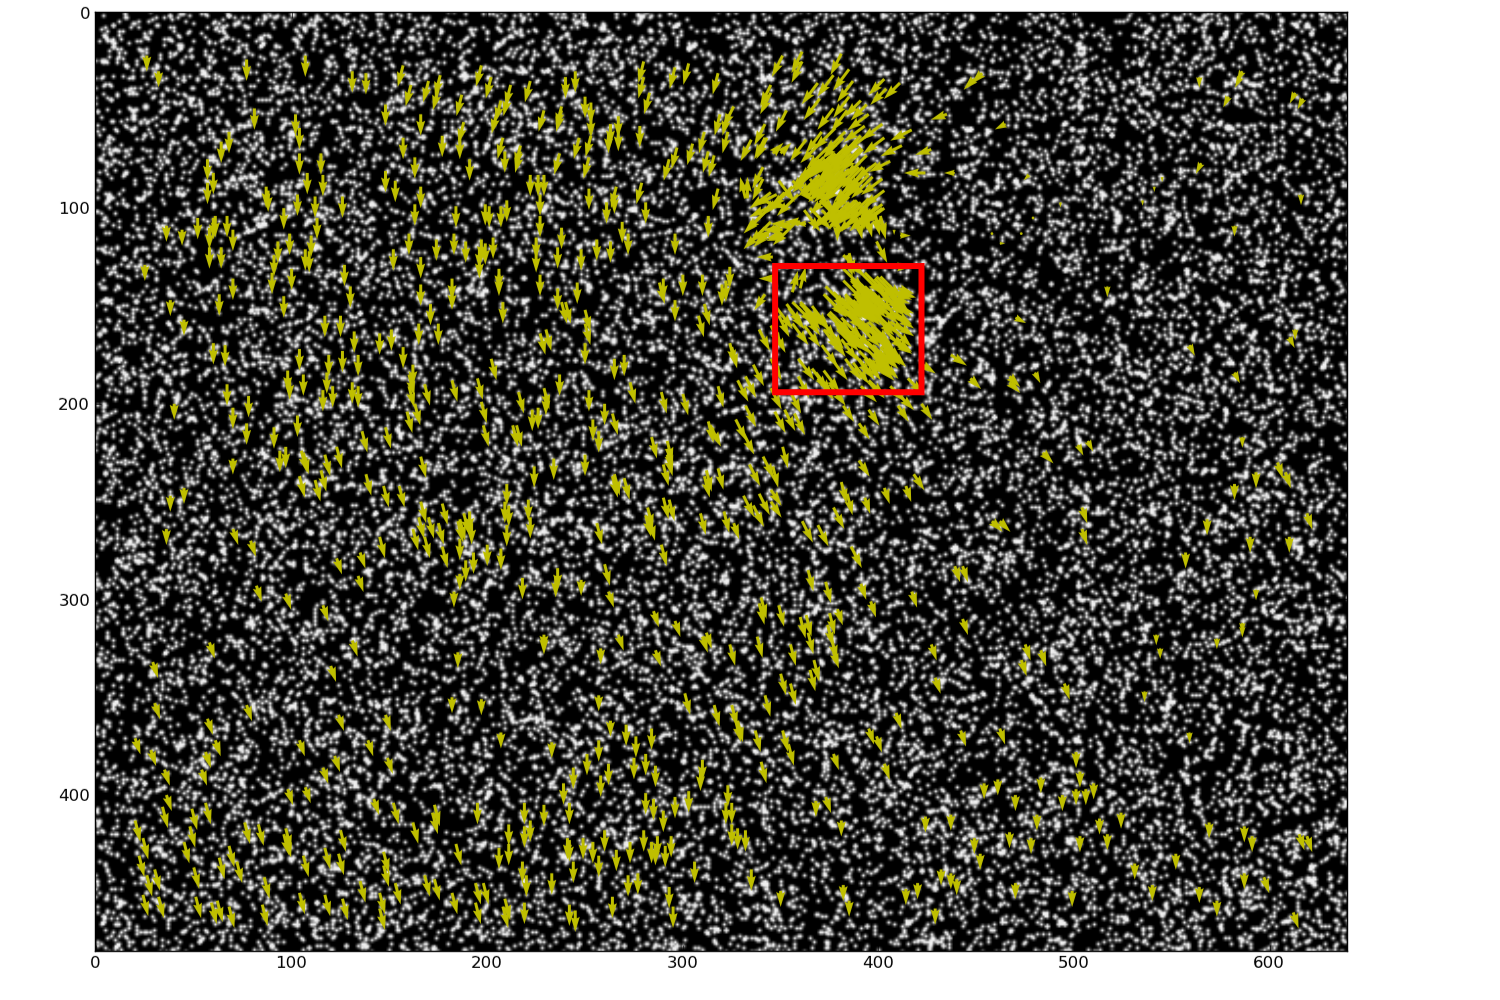
\includegraphics[width=\textwidth]{fig/adaptive_1000_zoomed_out_box.png}
	\end{subfigure}
	\begin{subfigure}[htb]{0.6\textwidth}
		\centering
		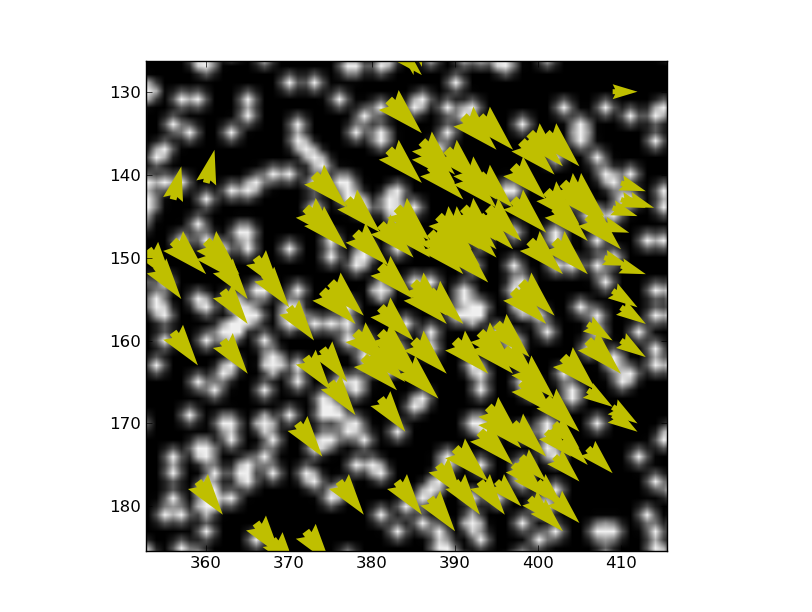
\includegraphics[width=\textwidth]{fig/adaptive_1000_detail.png}
	\end{subfigure}
	\caption{Results of adaptive PIV using the sampled interrogation window locations shown in Figure \ref{fig:distribution}. The area within the red box in (a) is shown in (b).}
	\label{fig:adaptive} 
\end{figure}

\section{Implementation Results}
I have successfully implemented the design described in this report to meet most of the goals described. I have demonstrated PIV tracking in simulation on images of 80x60, 640x480, and 800x600 pixels with up to 40 parallel Window Trackers. I have also synthesized and run the design on hardware with image sizes up to 640x480 pixels and 2 parallel trackers. 

\subsection{Performance on Hardware}
\label{sec:performance}
The results of this project are promising but do not yet meet the full targets for performance. I ran a series of benchmark tests to determine the effectiveness of parallelizing the design to multiple Window Tracker modules. With a single tracker module, the system completed 18,000 window requests in 30.8\,seconds, for an overall rate of $4.85 \times 10^7$ multiplications per second, or almost exactly one multiplication per clock cycle. With two parallel trackers, 18,000 requests took only 15.7\,s, for a rate of $9.49\times10^7$ multiplications per second or 1.9 multiplications per clock cycle. This is extremely close to the target rate of 1 multiplication per cycle per module. 

Unfortunately, this performance does not yet scale properly beyond two parallel trackers, and adding more modules does not significantly improve the execution speed. This is likely due at least in part to contention for the single main Block RAM, which must serve out the sub-frames to each tracker. 

\subsection{Implementation Challenges}
There were a number of problems encountered in the design process, primarily when attempting to use the design on the FPGA. When I restricted the size of the images to 80x60 pixels, I was able to implement at least 40 parallel tracking modules (although they did not necessarily improve execution speed, as discussed previously). However, when I upgraded the system to 640x480 or 800x600 pixels, I began having a number of difficulties. With 800x600 pixels, I was using 91\% of available Block RAMs and synthesis reported success, but the design would not run. Removing the reset transactor and ensuring that there were no SceMi transactors passing void messages removed some of the hangups experienced in execution but did not allow me to successfully run the system with more than two trackers. 

\subsection{Device Utilization}
Timing was not an issue with this design, as the timing analysis consistently reported maximum frequencies of over 60\,MHz. The primary constraint for implementation was Block RAM usage. With an image size of 640x480, 60\% of RAMs were used, and with 800x600 images over 90\% of available RAMs were in use. 

\subsection{Bluespec Code and IP Reuse}
The image memory module used to store each frame for PIV analysis was based on the IMemory and DMemory used in the SMPIPS processor implementation. The Ehr, Vector, and FIFO implementations were also used throughout the design. All told, there were approximately 700 lines of Bluespec used in this design, with a few hundred more lines of supporting C++ and Python code. 

\section{Future Explorations}
I would like to extend the design to support varying the size of the interrogation window. This is an important part of the Adaptive PIV algorithm, as it allows the system to examine smaller windows of particle flow in busy areas of the image, in which the assumption that all particles within a window are moving with the same velocity might not hold for a larger window. This will require adding a window size parameter to the reset() method of the Window Manager and will require that that size parameter be passed to the Accumulator and Tracker in order to adjust their behavior accordingly. 

In addition, I would like to explore ways to overcome the parallelization limits I encountered. The most likely next step in that exploration would be to improve the efficiency of access to the primary image Block RAMs. One possible method would be to store multiple pixels per word in RAM, which would allow multiple pixels to be retrieved per cycle. Alternatively, I could duplicate the Block RAMs to allow parallel access. 

\section{Conclusion}
This paper presents a functioning implementation of Particle Image Velocimetry, which is sufficiently flexible to perform standard PIV or a form of adaptive PIV in which the spatial frequency of the interrogation windows is adjusted while their size remains the same. It achieves a throughput rate of 1 multiplication per cycle per tracker, which will be sufficient to allow real-time PIV imaging if it can be extended to 40 parallel modules. 

	\bibliographystyle{plain}
	\bibliography{refs}
\end{document}